Embarking on the findings of this chapter, we transition from the established COMSOL modeling workflow to the critical stage of validating theoretical concepts through the lens of computational analysis. The essence of this chapter is twofold: first, to harness the computational prowess of COMSOL in substantiating key optical phenomena such as anti-reflectivity thus corroborate our simulation outcomes with theoretical models; and second, to attempt to model the simplest Passive Daytime Radiative Cooling devices (PDRCs) at Hudgings Lab by showing how their reflectance varies with wavelength.

Our investigation begins with an empirical analysis of anti-reflective behaviors, examining both simple and composite multilayer arrangements. These simulations are meticulously compared to the theoretical predictions presented in \emph{Introduction to Optics} by Frank L. Pedrotti et al., ensuring our findings adhere to the rigorous standards of optical precision.

We delve into the intricacies of high reflectance by simulating stacks of alternating high and low refractive index layers, shedding light on the nuanced ways layer configurations impact reflectance. These insights are bench-marked against scholarly literature, reinforcing the accuracy of our models.

Aligning with practical applications, we employ the Fresnel equations to map out the reflection coefficient, for both the transverse electric (TE) and transverse magnetic (TM) polarization, against the angle of incidence. The insights gleaned here will serve to consolidate our understanding of various optical phenomena.

Moreover, the thesis explores the layered design of PDRCs. By systematically layering glass, silver, and Polydimethylsiloxane (PDMS), we dissect the optical properties crucial to the development of passive cooling systems.

This chapter stands at the intersection of physics and simulation, merging the realms of theory and experimentation. The collection of results and graphs here encapsulate more than just data; they are catalysts for continuous inquiry and deeper understanding of optical physics as it related to PDRCs.

\section{COMSOL: Modeling Anti-reflectivity.}
Recall, per equation \ref{reflectance for 2-layer antireflecting films}, assuming normal incidence that

\begin{equation}\label{reflectance for 2-layer antireflecting films - chap4}
    R = \left(\frac{n_0n_2^2 - n_sn_1^2}{n_0n_2^2 + n_sn_1^2}\right)^2
\end{equation}
Zero reflectance is expected when the numerator is zero which results in \ref{zero reflectance criterion}
\begin{equation}\label{zero reflectance criterion - chap4}
    \frac{n_2}{n_1} = \sqrt{\frac{n_s}{n_0}}
\end{equation}

For a glass substrate with a refractive index of $n_s = 1.5$ and incidence for air with refractive index of $n_0 = 1$, the optimal ratio of the refractive indices, $\frac{n_2}{n_1} = \sqrt{1.5} \approx 1.225$, therefore in COMSOL we need to define and choose two materials, for our double layer, such that the ratio, $\frac{n_2}{n_1}$ is as close to 1.225 as possible, this way we can achieve optimal anti-reflectivity. As a reminder, in the visible spectrum, which ranges approximately from 400 to 700 nm, each wavelength interacts differently with the optical materials based on their refractive index at that specific wavelength. The optimal thickness and refractive index that reduce reflectance for one wavelength will not necessarily be optimal for another due to this dispersion and it is also difficult to choose 2 or more materials such that the combination of their refractive indices is so precise that the reflectance emerges to be exactly zero, so we can only hope to arrive to as close as 0\% reflectance but not exactly at 0\%.

Another drawback of the quarter-wavelength layer is that while it can prevent reflection of light at one wavelength, it reflects a substantial amount of radiation at any other nearby wavelength. The reflectance of the quarter-wavelength layer also depends heavily on the angle of incidence of the light. An alternative is to use a coating that consists of multiple layers. Compared to single-layer coatings, a multilayer coating is more likely to reduce the reflection coefficient across a band of wavelengths and can be produced using a wider variety of real materials.
In this the next section we'll show, the reflectance of two different multilayer coatings is compared over a wide spectral range: a quarter-quarter coating (two layers), and a quarter-half-quarter coating (three layers). The quarter-half-quarter coating is shown to have more consistently low reflectance across most of the visible spectrum. % TODO: CITE the Anti-Reflective Coating with Multiple Layers Tutorial and REPHRASE

% TODO: Change the title of this subsection

\subsection{Anti-reflectance Layers - not in book}

You need to model the layers as thin film dielectrics in COMSOL. To accurately emulate the zero reflectance criterion \ref{zero reflectance criterion - chap4}, I selected the first thin film dielectric (where I am counting from the bottom-up) to be cerium tri-fluoride ($\text{CeF}_3$) which has a refractive index of 1.63 and the second thin film dielectric to be magnesium fluoride ($\text{MgF}_2$) which has a refractive index of 1.38. The ratio of their refractive indices is thus $\frac{1.63}{1.38} \approx 1.181$ which is close to our desired ratio of 1.225. Recall that for modelling anti-reflectivity for a double layer as we saw in chapter 2, we need both layers to be of a quarter-wavelength thickness, where by this I mean the layers need to be a quarter of the wavelength we're evaluating the zero reflectance at, i.e., the wavelength where we want the reflectance to be at its most minimum. For the three-layer (quarter-half-quarter wavelength) model, which boosts anti-reflectivity across a wider range of wavelengths than the more restrictive quarter-quarter wavelength two-layer model, for the half-wavelength thin-film dielectric material, which sits in between the quarter-wavelength materials, I chose $\text{ZrO}_2$ which has a refractive index of 2.1.

Here is a snapshot of the COMSOL desktop which shows this. Notice the calculation of the quarter-wavelength in the ``Film Properties" section of the ``Thin Dielectric Film" settings:

% TODO: Add the image of the COMSOL desktop showcasing antireflectivity

% \begin{figure}[ht!]
%   \centering
%   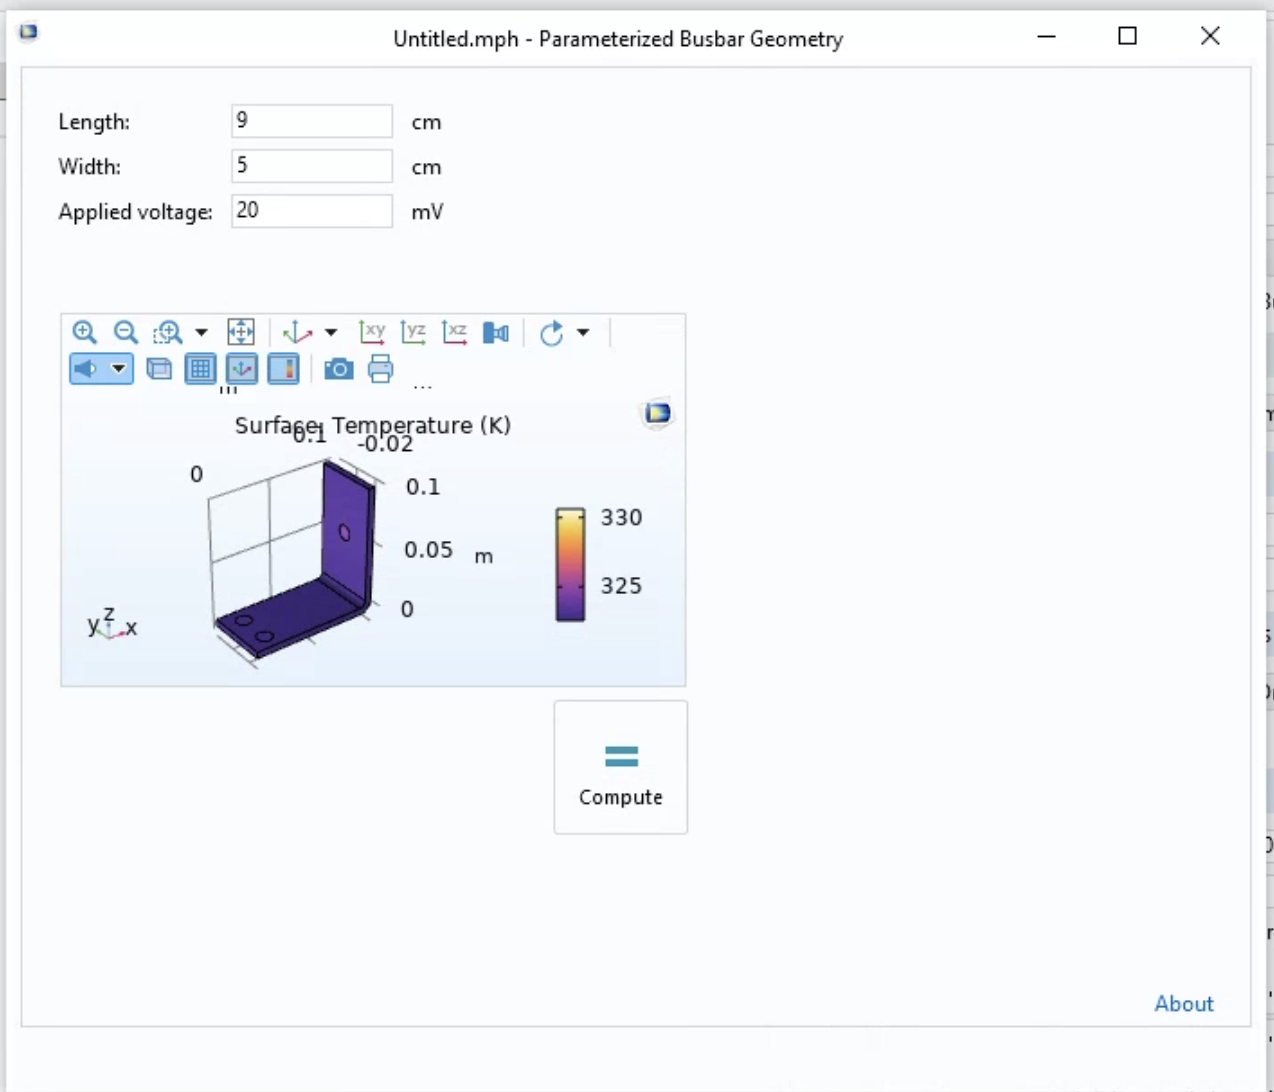
\includegraphics[width=0.4\textwidth]{Chapters/Figures/Chapter 3 Figures/Test Application Results.png}
%   \caption{Test Application button. Source: \cite{multiphysics__modeling_nodate}}
%   \label{fig:Test Application button.}
% \end{figure}

These are the results for modelling anti-reflectivity using $\text{CeF}_3$ and $\text{MgF}_2$ (as the quarter-quarter wavelength materials) and $\text{CeF}_3$, $\text{MgF}_2$, and $\text{ZrO}_2$ as the quarter-half-quarter wavelength materials respectively:

% TODO: Add the image of the anti-reflectivity results (from the tutorial) using CeF3 and MgF2 and ZrO2

% \begin{figure}[ht!]
%   \centering
%   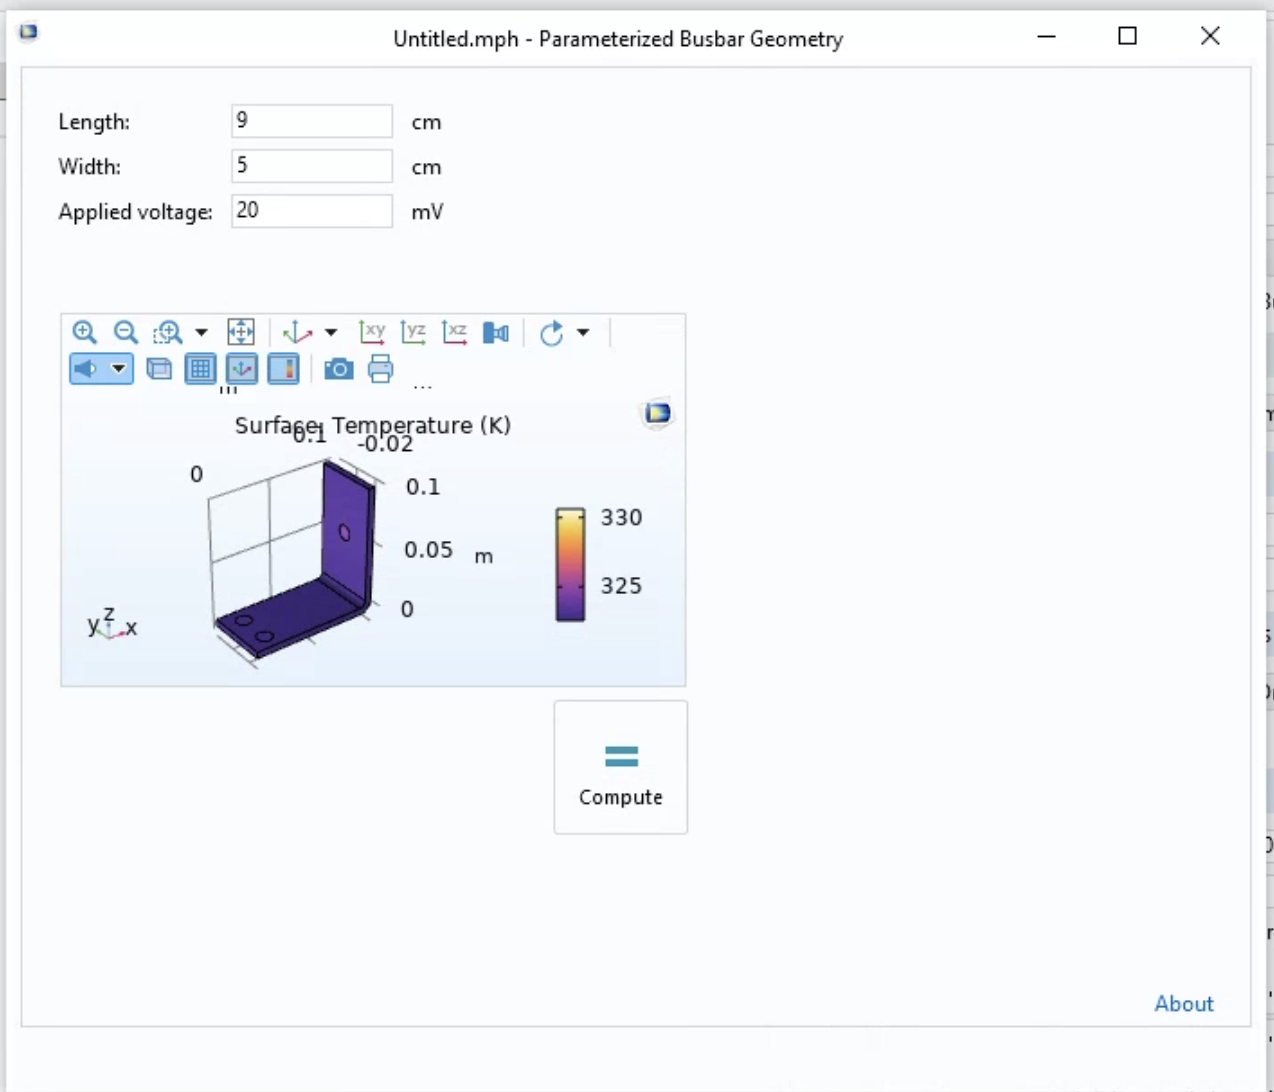
\includegraphics[width=0.4\textwidth]{Chapters/Figures/Chapter 3 Figures/Test Application Results.png}
%   \caption{The graph displays the reflective properties of two types of antireflective coatings over a range of wavelengths in the visible spectrum. The blue curve represents a quarter-quarter wavelength coating, while the green curve depicts a quarter-half-quarter wavelength coating. Source: \cite{multiphysics__modeling_nodate}}
%   \label{fig:Test Application button.}
% \end{figure}

For the quarter-quarter coatings, this configuration consists of two layers, each a quarter-wavelength thick. The ideal situation for such a coating is to have zero reflectance at a specific wavelength, but due to practical limitations of material properties, perfect zero reflectance is usually not achieved. For the quarter-half-quarter coating, adding a third layer, a half-wavelength thick, between the two quarter-wavelength layers forms this configuration. This setup is designed to reduce reflectance over a broader range of wavelengths.

The practical implication of this is that multi-layer coatings are more effective than single-layer ones for anti-reflective purposes, as they can address a range of wavelengths. This makes them suitable for various applications where reducing glare and maximizing light transmission are crucial, such as in lenses and optical devices.

% TODO: Change the title of this subsection

\subsection{Anti-reflectance Layers - Confirmation of book results.}

Next, we seek to replicate the theoretical underpinnings of multilayer films in the book \emph{Introduction to Optics} by Frank L. Pedrotti et al., ensuring our findings adhere to the rigorous standards of optical precision.

To start off simply, we choose to plot reflectance from a double-layer film versus wavelength for these three cases:
\begin{itemize}
    \item Quarter-quarter wavelength films.
    \item Quarter-half wavelength films.
    \item Quarter-half wavelength films (using a different material for the half-wavelength coating).
\end{itemize}

% TODO: Add figure 5 (Antireflecting double layer using l>4–l>2 thickness films. Reflectance curves are shown in Figure 4.)

% \begin{figure}[ht!]
%   \centering
%   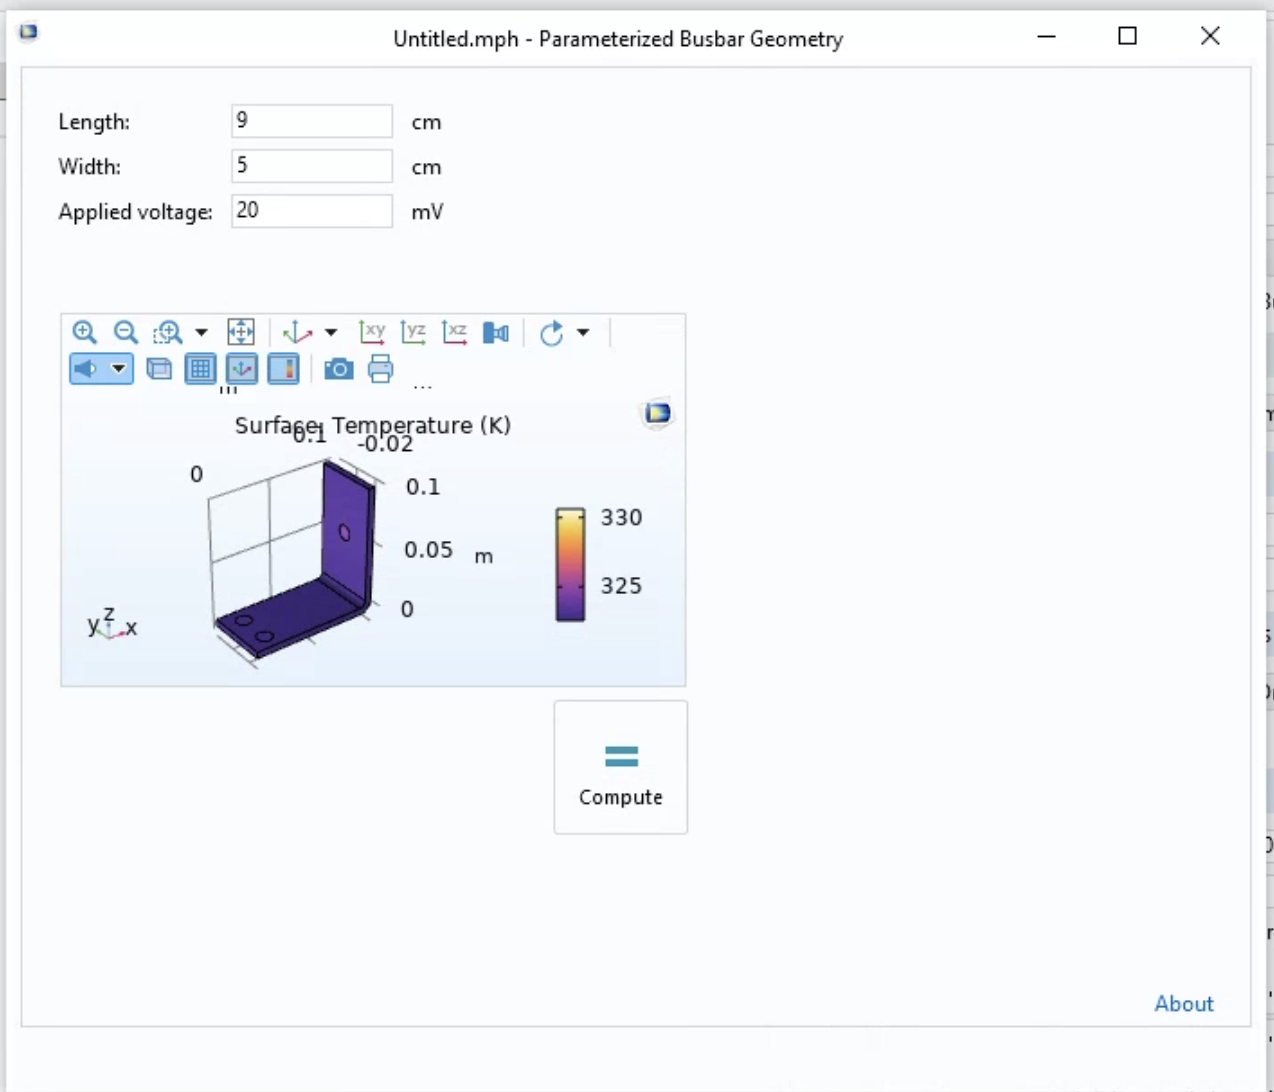
\includegraphics[width=0.4\textwidth]{Chapters/Figures/Chapter 3 Figures/Test Application Results.png}
%   \caption{Test Application button. Source: \cite{multiphysics__modeling_nodate}}
%   \label{fig:Test Application button.}
% \end{figure}

Let's start with the quarter-quarter wavelength films. The book uses the first thin dielectric film from the bottom as $\text{ZrO}_2$ and the second thin dielectric film as $\text{CeF}_3$ just above the $\text{ZrO}_2$ layer. Of course, as long as \ref{zero reflectance criterion - chap4} holds, we can use any 2 materials such that the ratio of their refractive indices is optimal for anti-reflectivity. In this case, the theory says, that $\frac{n_2}{n_1} = \frac{2.1}{1.65} \approx 1.273$. This is close to the optimal ratio of 1.225 we would like to have assuming that $n_s = 1.5$ and that the angle of incidence is normal.

Broader regions of low reflectance also become possible in the visible region of the spectrum, once the restriction of using equal $\lambda/4$ coatings is relaxed. Therefore, we can use a quarter-wavelength thick layer as the second layer (bottom up) to ensure broader regions of low reflectance. Thus for item b, the quarter-wavelength thick material is $\text{MgF}_2$ which has a refractive index of 1.38 and the half-wavelength thick material is made of aluminum oxide which has a refractive index of 1.60 while that of item (c) is made of thorium dioxide which has a refractive index of 1.85. % TODO: CITE PEDROTTI

At the wavelength of 550 nm, for which the $\lambda/4$ and $\lambda/2$ thicknesses are determined, the $\lambda/2$ layer has no effect on the reflectance and the double layer behaves like a single $\lambda/4$ layer with $R = 1.3\%$. At nearby wavelengths, the $\lambda/2$ layer helps to keep $R$ below values attained by a single $\lambda/4$ layer alone. Here is the combined reflectance versus wavelength plot for scenarios (a) through (c):

% TODO: Add the antireflectivity graphs in the Optics book.

% \begin{figure}[ht!]
%   \centering
%   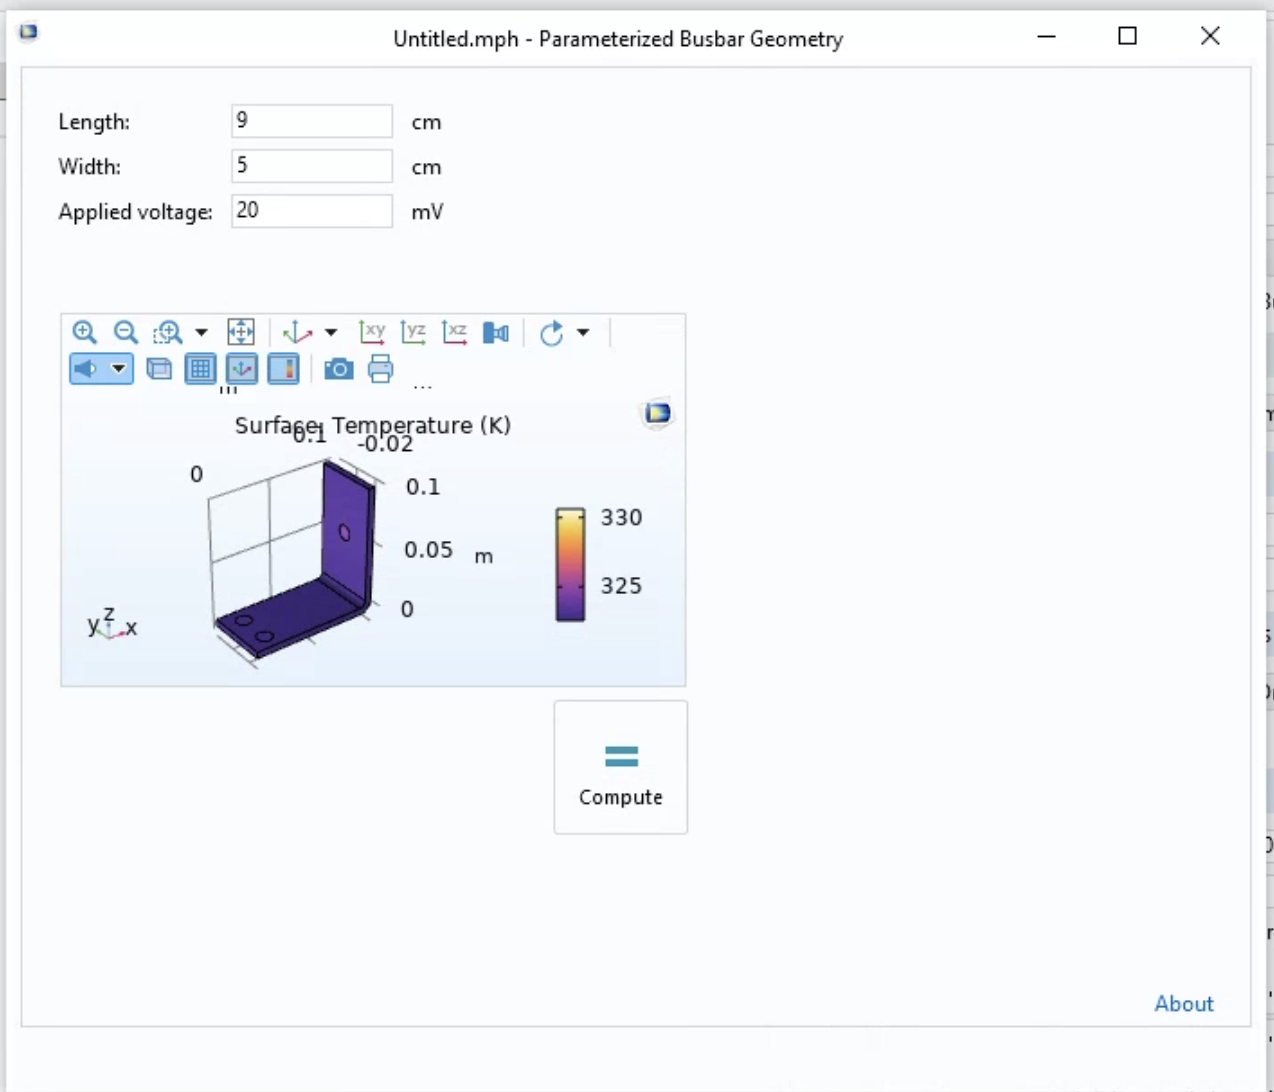
\includegraphics[width=0.4\textwidth]{Chapters/Figures/Chapter 3 Figures/Test Application Results.png}
%   \caption{Test Application button. Source: \cite{multiphysics__modeling_nodate}}
%   \label{fig:Test Application button.}
% \end{figure}

Although reflectance at 550 nm is about 1.3\%, greater than for the $\lambda/4$- $\lambda/4$ coating, it remains at values less than this over the broad range of wavelengths from about 420 to 800 nm. Other practical solutions for double layer reflecting films become possible if the thicknesses of the layers are allowed to have values other than multiples of $\lambda/4$.

Below are my attempts to model all 3 scenarios (a), (b), and (c) itemized above.

% TODO: Add my own antireflectivity graphs
% TODO: Add graph (a)

% \begin{figure}[ht!]
%   \centering
%   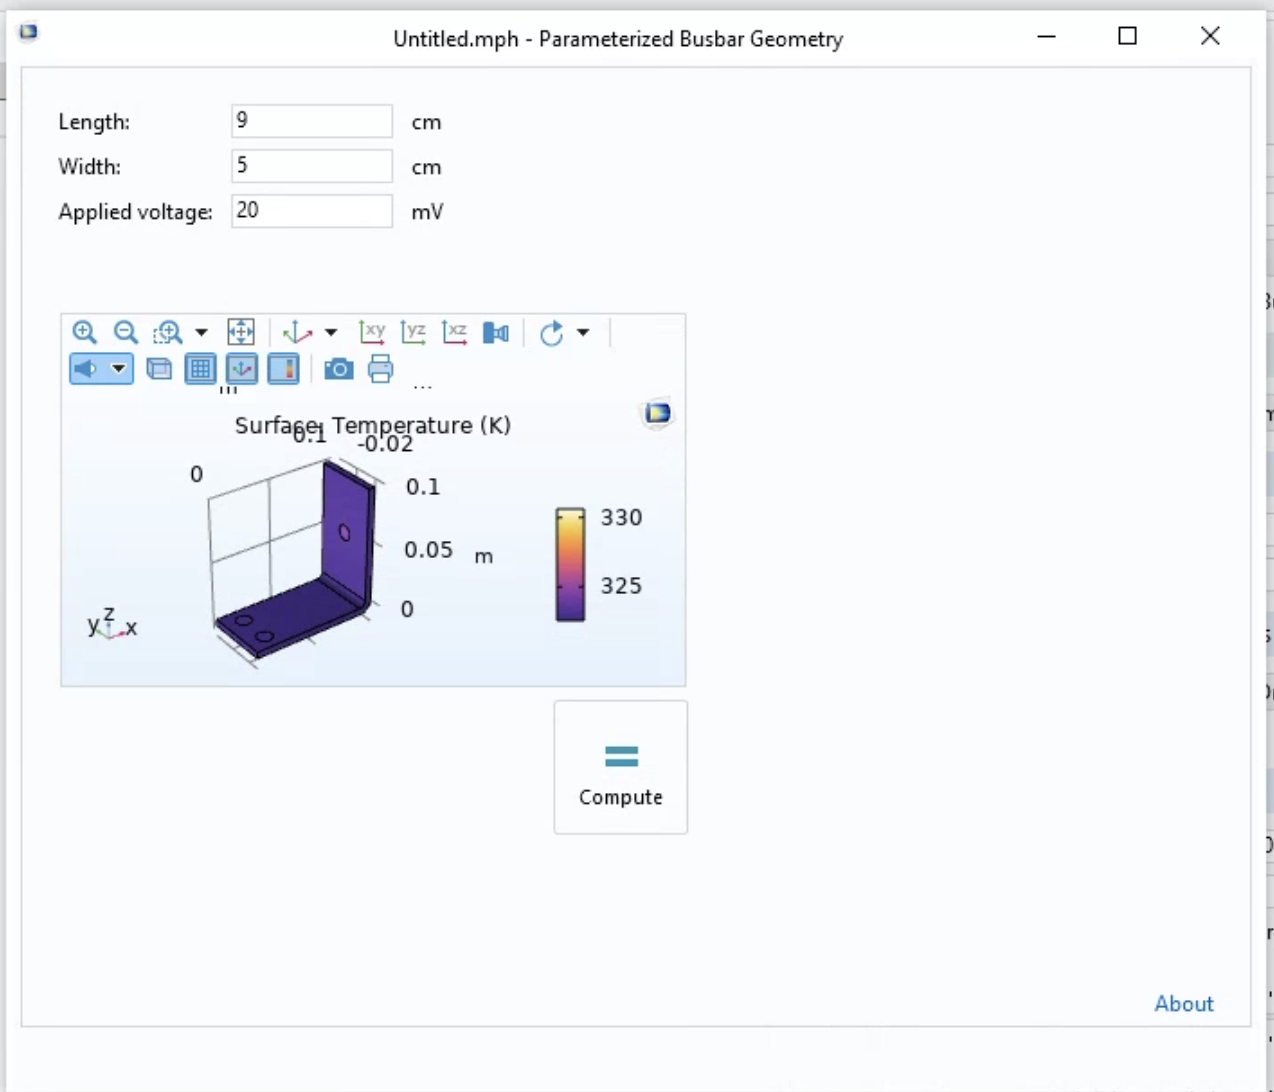
\includegraphics[width=0.4\textwidth]{Chapters/Figures/Chapter 3 Figures/Test Application Results.png}
%   \caption{Test Application button. Source: \cite{multiphysics__modeling_nodate}}
%   \label{fig:Test Application button.}
% \end{figure}

% TODO: Add the antireflectivity graphs in the Optics book.
% TODO: Add graph (b)

% \begin{figure}[ht!]
%   \centering
%   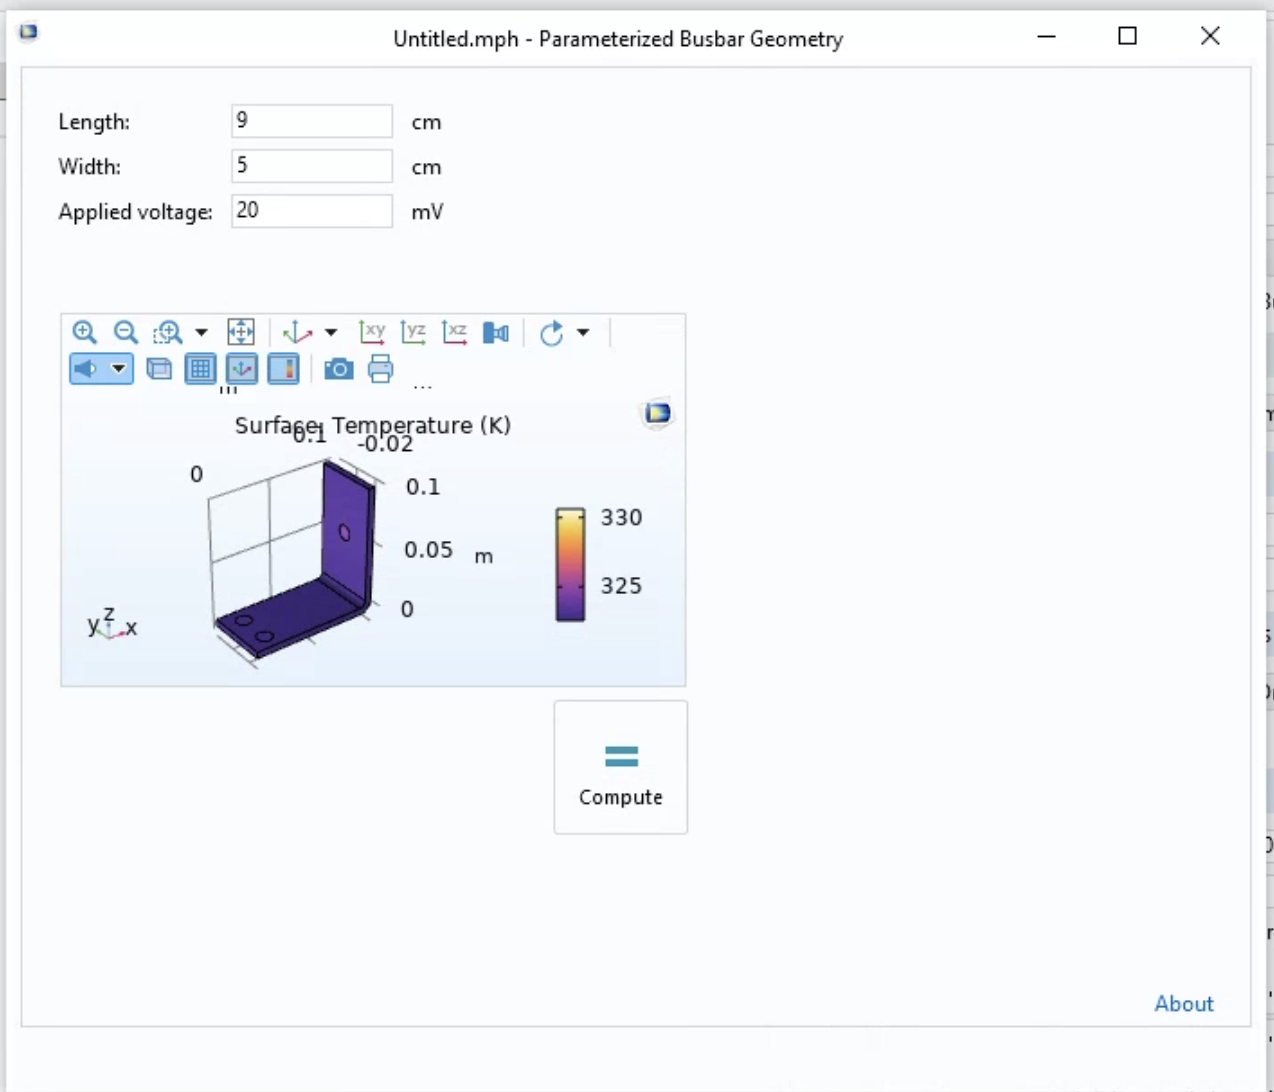
\includegraphics[width=0.4\textwidth]{Chapters/Figures/Chapter 3 Figures/Test Application Results.png}
%   \caption{Test Application button. Source: \cite{multiphysics__modeling_nodate}}
%   \label{fig:Test Application button.}
% \end{figure}

% TODO: Add the antireflectivity graphs in the Optics book.
% TODO: Add graph (c)

% \begin{figure}[ht!]
%   \centering
%   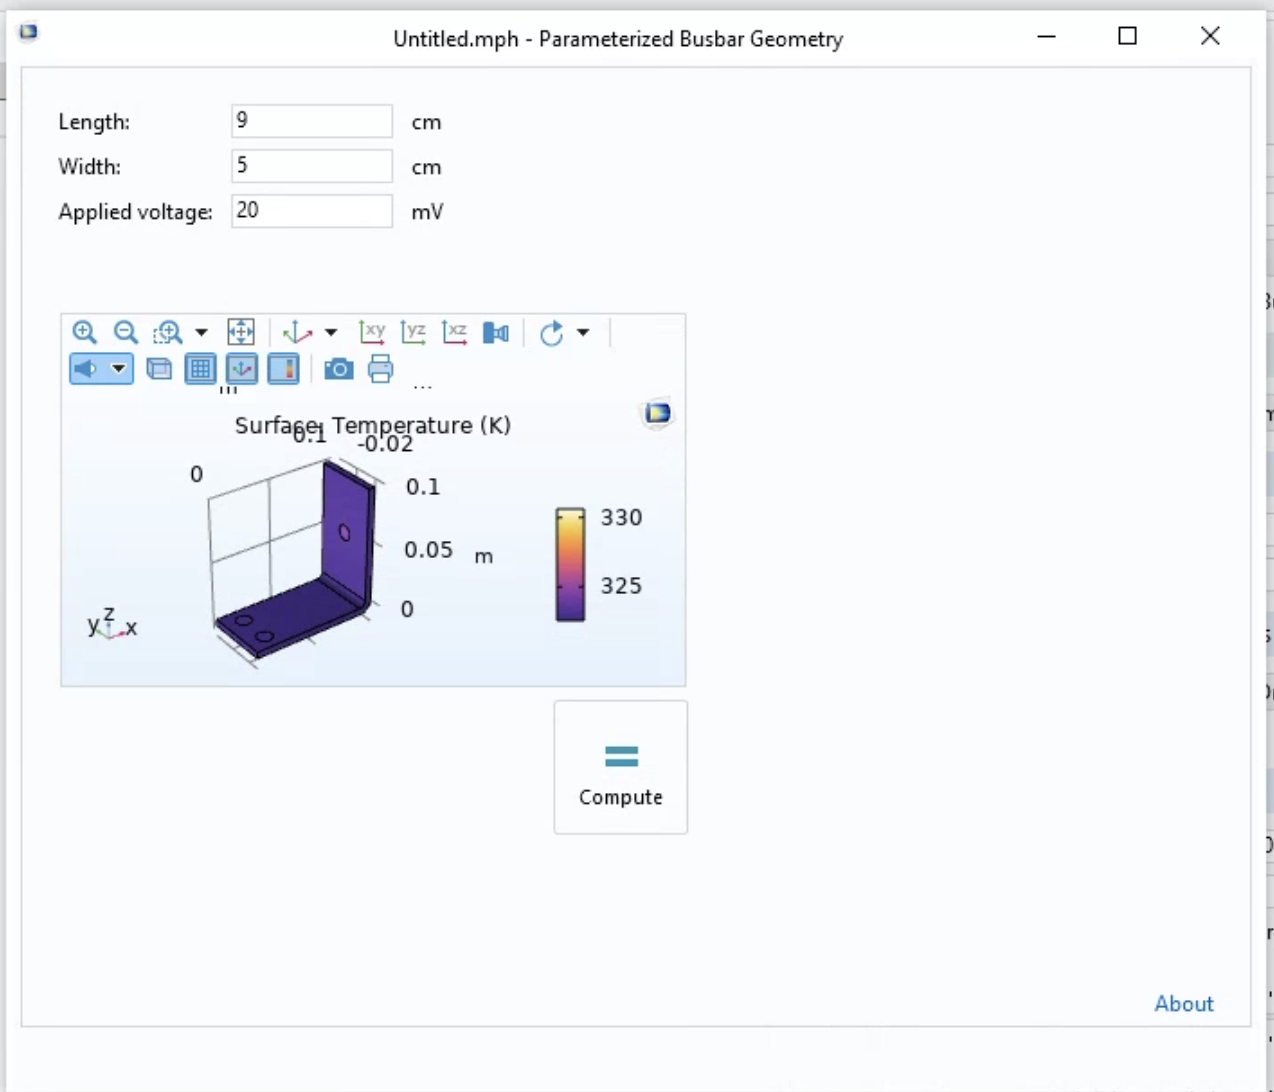
\includegraphics[width=0.4\textwidth]{Chapters/Figures/Chapter 3 Figures/Test Application Results.png}
%   \caption{Test Application button. Source: \cite{multiphysics__modeling_nodate}}
%   \label{fig:Test Application button.}
% \end{figure}

The 3 curves above have been calculated using the theory presented in chapter 2. The overall transfer-matrix elements are first determined by forming the product of the transfer matrices of the individual layers. In these elements, the phase difference, $\delta$, is expressed as a function of $\lambda$, and the film thickness is determined by the $\lambda/4$ or $\lambda/2$ requirement at a single wavelength (550 nm).

The matrix elements can then be used to calculate the reflection coefficient given in \ref{reflection coefficient in terms of transfer matrix terms} so when squared given the reflectance as a function of wavelength. Thankfully, COMSOL, in particular, the Ray Optics package helps in doing semi-automatically, with few probings, such as how to treat the layers (which in this case, we should treat the layers as thin dielectric films).